% ****** Start of file aipsamp.tex ******
%
%   This file is part of the AIP files in the AIP distribution for REVTeX 4.
%   Version 4.1 of REVTeX, October 2009
%
%   Copyright (c) 2009 American Institute of Physics.
%
%   See the AIP README file for restrictions and more information.
%
% TeX'ing this file requires that you have AMS-LaTeX 2.0 installed
% as well as the rest of the prerequisites for REVTeX 4.1
% 
% It also requires running BibTeX. The commands are as follows:
%
%  1)  latex  aipsamp
%  2)  bibtex aipsamp
%  3)  latex  aipsamp
%  4)  latex  aipsamp
%
% Use this file as a source of example code for your aip document.
% Use the file aiptemplate.tex as a template for your document.
\documentclass[%
 aip,
% jmp,
% bmf,
% sd,
% rsi,
 amsmath,amssymb,
%preprint,%
 reprint,%
%author-year,%
%author-numerical,%
% Conference Proceedings
]{revtex4-1}

\usepackage{graphicx}% Include figure files
\usepackage{dcolumn}% Align table columns on decimal point
\usepackage{bm}% bold math
%\usepackage[mathlines]{lineno}% Enable numbering of text and display math
%\linenumbers\relax % Commence numbering lines

\usepackage[utf8]{inputenc}
\usepackage[T1]{fontenc}
\usepackage{mathptmx}
\usepackage{etoolbox}
\usepackage{mathtools}
\usepackage{amsfonts}
%% Apr 2021: AIP requests that the corresponding 
%% email to be moved after the affiliations
\makeatletter
\def\@email#1#2{%
 \endgroup
 \patchcmd{\titleblock@produce}
  {\frontmatter@RRAPformat}
  {\frontmatter@RRAPformat{\produce@RRAP{*#1\href{mailto:#2}{#2}}}\frontmatter@RRAPformat}
  {}{}
}%
\makeatother
\newcommand{\cchevrons}[1]{\langle\!\langle #1 \rangle\!\rangle}
\DeclarePairedDelimiter\abs{\lvert}{\rvert}
\DeclarePairedDelimiter\norm{\lVert}{\rVert}
\begin{document}

\preprint{AIP/123-QED}

\title[]{A kinetic interpretation of the Frank's constants in calamitic fluids}
% Force line breaks with \\
\author{P. E. Farrell}
\author{U. Zerbinati}
 %\altaffiliation[Also at ]{Physics Department, XYZ University.}%Lines break automatically or can be forced with \\
%\author{B. Author}%
 %\email{Second.Author@institution.edu.}
%\affiliation{ 
%Authors' institution and/or address%\\This line break forced with \textbackslash\textbackslash
%}%

%\author{C. Author}
 %\homepage{http://www.Second.institution.edu/~Charlie.Author.}
%\affiliation{%
%Second institution and/or address%\\This line break forced% with \\
%}%
\date{\today}% It is always \today, today,
             %  but any date may be explicitly specified

\begin{abstract}
\end{abstract}

\maketitle

\section{\label{sec:intro}Introduction}
In Ref.~\onlinecite{FRZ23} a kinetic approach to obtain hydrodynamic equations for calamitic fluids has been investigated, with the aim to derive an inviscid and compressible variant of the well-kown Leslie-Eriksen equations.
In the process, a kinetically motivated variant energy for the orientational degrees of freedom was proposed, in the absence of extern-field i.e.
\begin{equation}
\label{eq:OseenFrankGen}
\mathcal{I}[\vec{n}]\coloneqq \int_{\Omega} \cchevrons{\vec{\omega} \cdot \mathbb{I}\vec{\omega}}\,d\vec{x},
\end{equation}
where $\mathbb{I}$ is the microscopic inertia tensor and the symbol $\cchevrons{\cdot}$ denotes the average over the microscopic: linear momentum $\vec{p}$, euler angles $\vec{\alpha}$ and their conjugate moments $\vec{\varsigma}$, weighted by the a priori unknown one-particle distribution $f(\vec{q},\vec{p},\vec{\alpha},\vec{\varsigma},t)$, i.e.~
\begin{equation}
	\cchevrons{\cdot} \coloneqq \frac{1}{n}\int\!\!\!\int\!\!\!\int\psi\,f({\vec{q}},\vec{p},\vec{\alpha},\vec{\varsigma},t)\,d\vec{v}d\vec{\alpha}d\vec{\varsigma}.
\end{equation}
Notice that phase-space, which variable we here denote $\Gamma=(\vec{\xi},\vec{\pi})=(\vec{q},\vec{p},\vec{\alpha},\vec{\varsigma})$, over which the one-particle distribution is evaluated is larger compared to the one for the classical Boltzmann equation, this because rotational degree of freedom $\vec{\alpha}$ and their conjugate moments $\vec{\varsigma}$ had to be considered in order to describe the configuration of a calamitic molecule.

Near the thermodynamical equilibrium we can evaluate $\cchevrons{\vec{\omega}\cdot \mathbb{I}\vec{\omega}}$ using the Maxwell-Boltzmann distribution, i.e. the one-particel $f^{(0)}(\vec{\alpha},\vec{v},\vec{\varsigma})$ distribution such that the collision operator vanish.
The Maxwell-Boltzmann distribution for calamitic molecules can be dervied from microscopical consideration to be,
\begin{equation}
  \label{eq:MaxwellBoltzmann}
  f^{(0)}(\vec{\alpha},\vec{V},\vec{\Omega})=\frac{m^{\frac{3}{2}}(I_1I_2I_3)^{\frac{1}{2}}}{(2\pi k_B T)^3}\exp\Big[-m\frac{\abs{\vec{V}}^2}{2 k_B T}-\frac{\vec{\Omega}\cdot\mathbb{I}\vec{\Omega}}{2k_B T}\Big]
\end{equation}
normalised multiplyinng by $\frac{nQ\sin(\alpha_2)}{\int_{\mathbb{R}^3}Q\sin(\alpha_2)\,d\alpha}$ where $Q$ is defned as 
\begin{equation}
  Q=\exp\left(\frac{\vec{\omega}_0\cdot \mathbb{I}\vec{\omega}_0}{\frac{2}{3}\cchevrons{\theta}}\right)
\end{equation}
and both $\omega_0$ and the kinetic temperature $T$ are assumed to remain constant at equilibrium\cite{C56,CD63}.

A well-known result in kinetic theory is that the Maxwell-Boltzmann distribution can be rewritten in terms of the microscopic collision invariants alone\cite{FM}, hence the only order parameters appearing in the energy $\mathcal{I}$ must come from the $\mathbb{I}$.
To see this let us consider first the excluded volume interaction potential $\vec{U}(\vec{q}_1,\vec{q}_2,\vec{\alpha}_1,\vec{\alpha}_2)$, which is well-known to conserve:
\begin{enumerate}
  \item the total linear momentum, i.e. $p$,
  \item the angular momentum, i.e. $\frac{1}{m}(\vec{q}\times \vec{p})+\mathbb{I}\vec{\omega}(\vec{\alpha},\vec{\varsigma})$,
  \item the total kinetic energy, i.e. $\frac{1}{2m}\vec{p}\cdot \vec{p}+\frac{1}{2}\vec{\omega}(\vec{\alpha},\vec{\varsigma})\cdot \mathbb{I}\vec{\omega}(\vec{\alpha},\vec{\varsigma})$.
\end{enumerate}
When considering an excluded volume interaction, thanks to the nature of the microscopic collision invariants it is trivial to see that the order parameter only plays a role in $\mathbb{I}$.
Interestingly enough the above-defined collision invariants are also the invariants for any two-body interaction occurring as a result of a radial and orientationally invariant intermolecular potential, as for example the Gay-Berne potential\cite{GB81}.
In fact the Lagrangian of this two-body interaction
\begin{align}
  \mathcal{L}(\vec{\Gamma}_1,\vec{\Gamma}_2)=\frac{1}{2m}(p_1^2+p_2^2)&+\frac{1}{2}\vec{\omega}_1(\vec{\alpha}_1,\vec{\varsigma}_1)\cdot \mathbb{I}\vec{\omega}_1(\vec{\alpha}_1,\vec{\varsigma}_1)\nonumber\\
  &+\frac{1}{2}\vec{\omega}_2(\vec{\alpha_2},\vec{\varsigma}_2)\cdot \mathbb{I}\vec{\omega}_2(\vec{\alpha}_2,\vec{\varsigma}_2)\nonumber\\,
  &+U(\abs{\vec{q}_1-\vec{q}_2},\alpha),
\end{align}
is invariant under the translation and rotation hence applying Noether's theorem
\begin{equation}
  \label{eq:Noether}
  \frac{d}{dt}\left(\frac{\partial \mathcal{L}}{\partial \dot{\vec{\xi}}_{1,2}}\cdot G_i\right)=0, \qquad i=1,2,
\end{equation}
where $G_i$ are the generators of the translation and rotation group, i.e. $G_1=(1,1,0,0)$ and for an arbitrary unit-vector $\vec{n}$, $G_2=(\vec{n}\times \vec{q},\vec{n}\times\vec{q},1,1)$. In particular, we remark that \eqref{eq:Noether} with $G_1$ gives the conservation of the total linear momentum, while with $G_2$ the conservation of the total angular momentum.
Lastly, the conservation of the total kinetic energy is a direct consequence of the fact that the Lagrangian is time-independent and its kinetic energy portion is a homogeneous positive definite quadratic form of the generalized velocities\cite{FM}.
information
While at first, it might not appear obvious there are interesting consequences of the above observation. Not only the order parameters can come into play only through the inertia tensor, but for this reason the microscopic mechanism resulting in macroscopic anisotropic behavior in a calamitic fluid near the thermodynamical equilibrium is only determined by the geometrical about the calamitic constituents encoded in the inertia tensor.
\section{Needle-like molecules}
In Ref.~\onlinecite{FRZ23} a particular case of the energy \eqref{eq:OseenFrankGen} was considered in greater detail, i.e. the case of needle-like cilindircal molecules for which the inertia tensor can be written as
\begin{equation}
  \label{eq:InertiaTensor}
  \mathbb{I} \approx \lambda(I-\vec{n}\times \vec{n}),
\end{equation}
where $K\approx \mathcal{O}(\gamma h^2)$ for a needle-like molecule of length $h$ and $\vec{n}$ is the usual nematic director field. Under the assumption that the molecule is cylindrical we can use $\gamma\approx \frac{1}{12}$.
Under this hypothesis and using the Maxwell-Boltzmann distribution \eqref{eq:MaxwellBoltzmann} to evaluate the energy \eqref{eq:OseenFrankGen} near the thermodynamical equilibrium, it was shown\cite{FRZ23} that $\mathcal{I}$ can be written as
\begin{equation}
  \label{eq:OseenFrankOne}
  \mathcal{I}[\vec{n}]=\int_\Omega p\frac{\lambda}{2}\,\nabla\vec{n}:\nabla\vec{n}\,d\vec{x},
\end{equation}
where we have dropped all the non-spatially dependent terms and $p$ is the thermodynamical pressure exerted by the calamitic constituents of the fluid. Notice that under isobaric conditions \eqref{eq:OseenFrankOne} is the one-constant variant approximation of the well-known Oseen-Frank energy\cite{V}.
We would like to point out that \eqref{eq:OseenFrankOne} gives a very rudimental equation to compute the one-constant approximation $K$ of the Frank's constants, i.e.
\begin{equation}
  \label{eq:FrankConstant}
  K=\lambda p.
\end{equation}
Let us look at a few examples to see if \eqref{eq:FrankConstant} provides a good ``ball-park'' park estimate for $K$.

We begin by considering para-Azoxyanisole (PAA), which is a calamitic molecule known to form a nematic phase at sufficiently high temperatures.
From a steric point of view, PAA can be considered as a needle-like molecule with a length $h\approx 20 \overset{\circ}{A}$ and a diameter $d\approx 5 \overset{\circ}A$\cite{dGJ}.
Furthermore, PAA is a solid compound that when heated up forms a nematic liquid crystal phase around $120\,C^\circ$ and $1.6\cdot 10^{7} \text{Pa}$\cite{dGJ,DCJ71}.
Using \eqref{eq:FrankConstant} we can provide a rough estimate for $K$, i.e.
\begin{equation}
  K_{PAA} \approx 33.3 \cdot 1.6\cdot 10^{-13} \text{N} \approx 5.3\cdot 10^{-7} \,\text{dyn}.
\end{equation}
This value is in good agreement with the experimental value for which $K_1\approx 0.7\cdot 10^{-6}\,\text{dyn}$, $K_2\approx 0.43\cdot 10^{-6}\,\text{dyn}$ and $K_3\approx 1.7 \cdot 10^{-6}\,\text{dyn}$\cite{dGJ}.

We now consider N-(4-methoxybenzylidene)-4-butylaniline (MBBA), which is another calamitic molecule known to form a nematic phase at room temperature. MBBA can be considered as a needle-like molecule with a length $h\approx 70 \overset{\circ}{A}$ if regarded as a rigid cylindrical body\cite{CRB71}.
At atmospheric pressure, MBBA forms a nematic phase from $20\,C^\circ$ to $47\,C^\circ$, therefore using \eqref{eq:FrankConstant} we can provide a rough estimate for $K$, i.e.
\begin{equation}
  K_{MBBA} \approx 408.3 \cdot 1.01\cdot 10^{-15} \,\text{N}\approx 4.12\cdot 10^{-8} \, \text{dyn}. 
\end{equation}

Lastly, we consider 4-pentyl-4'-cyanobiphenyl (5CB), which can be regarded as a needle-like molecule with height $h\approx 20 \overset{\circ}{A}$\cite{Z} which forms a nematic phase from $22.5\,C^\circ$ to $35\,C^\circ$ at atmospheric pressure.
Hence once again using \eqref{eq:FrankConstant} we can provide a rough estimate for $K$, i.e.
\begin{equation}
  K_{5CB} \approx 33.3 \cdot 1.01\cdot 10^{-15} \,\text{N}\approx 3.3\cdot 10^{-8} \, \text{dyn}.
\end{equation}

\begin{figure}
  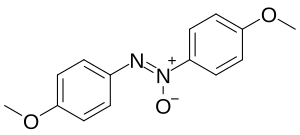
\includegraphics[scale=0.4]{Figures/PAA}\\
  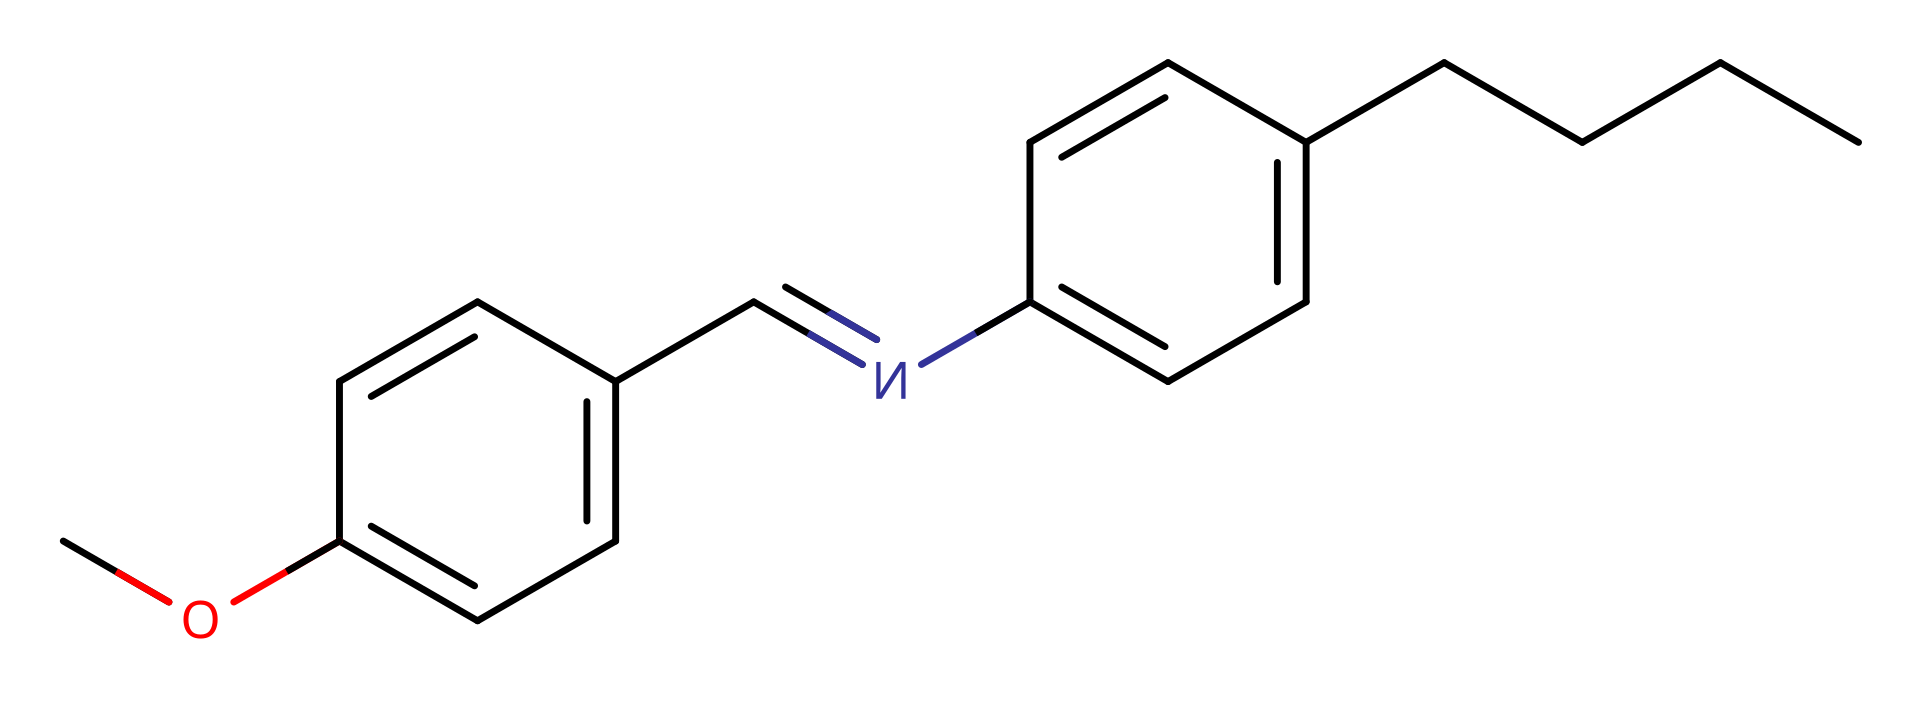
\includegraphics[scale=0.11]{Figures/MBBA}
  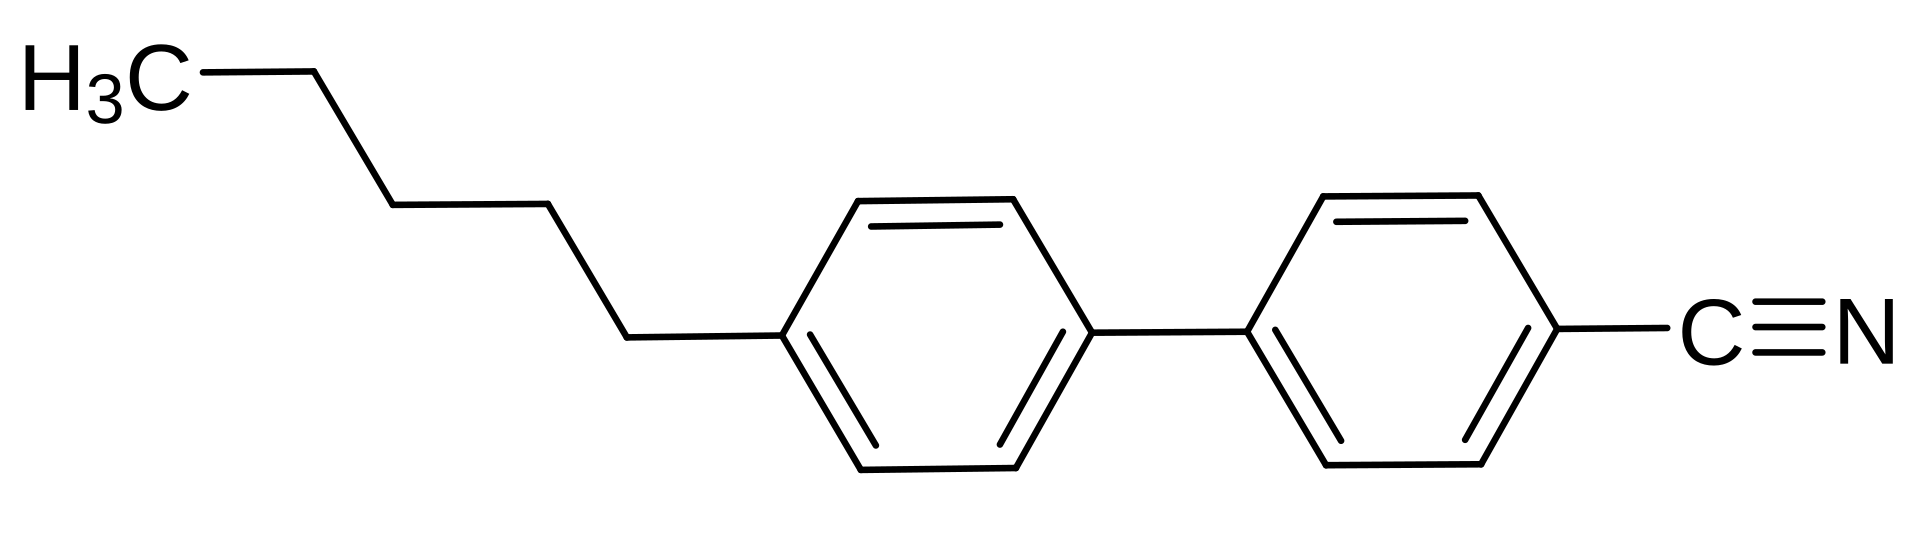
\includegraphics[scale=0.085]{Figures/5CB}
  \caption{In this figure are depicted the chemical structure of PAA, MBBA, and 5CB liquid crystal.}
  \label{fig:chem}
\end{figure}

While for PAA, \eqref{eq:FrankConstant} provided a good one constant approximation of Frank's constants, the same can not be concluded for MBBA and 5CB for which \eqref{eq:FrankConstant} understimates the Frank constant by one order of magnitude.
Looking at Figure \ref{fig:chem} a possible explanation comes to mind, i.e. while the chemical structure of PAA seems to be almost head-to-tail symmetric and therefore we can regard it as a needle-like cylinder the same can not be said for MBBA and 5CB.
One idea can be to regard MBBA and 5CB as needle-like cones, where the adjective needle-like refers to the fact that we assume \eqref{eq:InertiaTensor} still holds, yet since we are assuming the molecule has a cone shape $\gamma\approx\frac{3}{5}$.
Using this assumption we obtain,
\begin{equation}
  K_{MBBA} \approx 3.7 \cdot 10^{-7}\,\text{dyn}, \qquad K_{5CB}\approx 2.9\cdot 10^{-7}\,\text{dyn}.
\end{equation}
These values are more in line with the experimental measure of Frank's constants for MBBA, for which $K_1 \approx 5.3 \cdot 10^{-7}\,\text{dyn}$, $K_2 \approx 2.2 \cdot 10^{-7}\,\text{dyn}$, $7.5\cdot 10^{-7}\, \text{dyn}$\cite{dGJ}, and 5CB for which $K_1\approx 3.5\cdot 10^{-7}\,\text{dyn}$ and $K_3\approx 4.15\cdot 10^{-7}\,\text{dyn}$\cite{BRBF85}.
\section{Pressure and Temperature dependence}
An interesting consequence of \eqref{eq:FrankConstant} is that it predicts that the Frank constant will increase linearly with the pressure. A positive correlation between Frank's constants and pressure has been observed also experimentally\cite{SBF87}, in particular the experimental data presented in Ref. \cite{PRPH12} we can confirm the linear dependence describe by \eqref{eq:FrankConstant}, for the beding and splay constants.

On the other hand, it is a well-known fact that the magnitude of the Frank constants decreases as the temperature increases\cite{dGJ,G73}.
The different behaviors between temperature and pressure reveal an issue with the qualitative behavior expressed in \eqref{eq:FrankConstant}.
If one has to believe the ideal gas law, which was derived in Ref.~\onlinecite{FRZ23} from the kinetic theory of calamitic fluids, the pressure and temperature are positively related by the equation of state
\begin{equation}
  p = R \rho T. 
\end{equation}
Since most studies of the Frank constant are performed at a low Mach number, we can assume that the density $\rho$ is constant, hence the pressure and temperature are linearly related, hence as the temperature increases we should also see an increase in the pressure resulting in a greater value for the one-constant approximation.
This is in contrast with the experimental data, which shows that the Frank constants decrease as the temperature increases.
Two comments are to be made, first of all, it is well known that the ideal gas law fails to capture the behavior of many calamitic fluids\cite{YV78}. A common cure in statistical mechanics is to resort to a virial series to express the equation of state, i.e.
\begin{equation}
  \label{eq:virialExp}
  Z \coloneqq \frac{\beta p}{\rho} = 1 + \sum_{n=2}^\infty B_n\rho^n
\end{equation}
where $T$ is the temperature, $\rho$ the density and $\beta$ is defined as $\beta^{-1}\coloneq k_B T$ with $K_B$ being the Boltzmann constant.
The compressibility factor $Z$ expresses the deviation of a fluid from an ideal gas.
Since the compressibility factor and the coefficients $B_n$ are positive, it seems that \eqref{eq:virialExp} still dictates that even for a generalized equation of state as the temperature increases the pressure must increase as well. Therefore by \eqref{eq:FrankConstant} we should also observe an increase in the one constant approximation $K$.
Although \eqref{eq:virialExp} seems to be predicting a positive correlation between temperature and the one-constant $K$, multiplying \eqref{eq:virialExp} by the speed of sound $c$ we obtain
\begin{equation}
  Zc = \beta p \kappa_S = c + \sum_{n=2}B_n\rho^nc, \label{eq:compressibility}
\end{equation}
where $\kappa_S$ is the isoentropic compressibility. What \eqref{eq:compressibility} indicates that if the speed of sound is sufficiently large as it is in classical liquid crystal not only the nearly stationary regime are in the low Mach number regime but also the correlation between pressure, temperature and density can be neglected.
Hence with respect to their elastic behavior, we can treat liquid crystals as incompressible and consider the pressure as a Lagrange multiplier enforcing the fact that the density $\rho$ remains constant, hence decoupling the pressure from the temperature.
While \eqref{eq:FrankConstant} might still fail to capture the negative correlation between the temperature $T$ and the one-constant $K$, at least we know that in nearly incompressible fluids $K$ is not positively related to the temperature.

We would like to remark that the incompressibility assumption seems to be valid only at the microscopic length scale, which is the length scale that characterizes the elastic behaviour of the fluid.
In fact, at smaller length scales, such as the acoustic length scale, it is well known that liquid crystals can not be treated as incompressible since sound waves can propagate in such media\cite{MLS72}.
Interestingly enough theory based on an equation of state of the form of \eqref{eq:virialExp} has been very successful in explaining sound behavior in liquid crystal\cite{V09}.
In particular, in Ref.~\onlinecite{V09} the author bases his theory of nematoacoustic effects on the assumption that liquid crystals are Korteweg fluids hence they obey van der Waals equation of state, which via Taylor expansion can be recasted as 
\begin{equation}
  Z = 1 + (b-a\beta) \rho + \sum_{n=2}^\infty b^n\rho^n,
\end{equation}
where $a$ and $b$ are constants respectively expressing respectively the strength of molecular interactions and the excluded volume effects.

A primitive explanation for the negative correlation between the temperature $T$ and the one-constant $K$ can be attributed to microscopic changes in the molecular shape.
Intuitively one can imagine that at higger temperatures in order to maximize the entropy the length of the chemical bond in the calamitic fluid constituent is shortened, resulting in a smaller value of the geometric quantity $\lambda$ that inturns affects the value of $K$.
Yet these mechanics remain to be fully understood by the authors and can only be labeled as a conjecture for the moment being.

\section{Mean Square Distortion and Bragg peak}
While the one-constant approximation \eqref{eq:OseenFrankOne} is well known to be of limited use, so much so that it is sometimes called the poor-man energy functional\cite{dGJ}, \eqref{eq:OseenFrankOne} might provide qualitative information on the relation between the geometry of the microscopic constituents and macroscopic behavior of a calamitic liquid fluid.
Assuming that the sample of calamitic fluid can be treated to good approximation as two-dimensional, we can introduce an angle $\theta:\mathbb{R}^2\to [0,2\pi)$ describing the average orienatation of the calamitic constituents inplace of the nematic vector $\vec{n}$. Rewriting \eqref{eq:OseenFrankOne} in the frequency domain we obtain,
\begin{equation}
  \label{eq:frequencyDomain}
  \mathcal{I}[\theta] = \int \frac{\lambda}{2(2\pi)^3} p \abs{\theta(\xi)}^2 \xi^2 \,d\xi.
\end{equation}
Using the equipartition of energy theorem we have,
\begin{equation}
  k_BT = \lambda \xi^2 p \cchevrons{\abs{\theta(\xi)}^2},
\end{equation}
transforming back from the frequency domain the previous equation yields
\begin{equation}
  \label{eq:meanSquareDistortion}
  \mathbb{E}\left[\abs{\theta(\vec{x})}^2\right] = \frac{2}{(2\pi)^3}\frac{k_B T}{\lambda p} \int_{L^{-1}}^{\xi_c}\xi^{-2}\,d\vec{\xi}=\frac{k_B T}{\lambda p}\xi_c,
\end{equation}
where $\xi_c \approx 2\cdot 10^{-7} \,cm^{-1}$ is the largest wave vector after which the linear elastic theory breaks down and $L$ is the sample size.
What \eqref{eq:meanSquareDistortion} is suggesting is that as the molecular constituents of a calamitic fluid get more elongated $\lambda$ increases quadratically causing the mean-square distortion to decrease at the same rate.
Likewise, \eqref{eq:meanSquareDistortion} suggests that the mean-square distortion decreases linearly with the pressure.

We would like to briefly comment on these observations.
As molecules get more elongated they are less free to move, in fact for extremely elongated molecules even a small change in the orientation will result in many molecules overlapping with each other.
This is the reason why the mean-square distortion decreases as the molecular constituents get more elongated. 
The effect of the pressure on the mean-square distortion is more subtle to explain, yet we can imagine that as the pressure increases the molecules are packed closer to each other hence even if the overall space that can be occupied by the molecules increases a slight change in the orientation of a molecule will result in a greater number of molecules overlapping with each other.

The consequences of the microscopic geometric of the calamitic constituents on the macroscopic behavior of the fluid are not only limited to the mean-square distortion. In fact, once the nematic phase is established we can assume the density $\rho$ of the calamitic fluid has a periodic modulation, i.e. 
\begin{equation}
  \rho(\vec{x}) = \rho_0 + \rho_1\cos(\vec{n}_0\cdot \vec{x}+\theta),
\end{equation}
where $\rho_0$ is the isotropic density, $\rho_1$ is the amplitude of the modulation which is related to the geometry of the calamitic constituents, $\vec{n}_0$ is a reference director field.
A common quantity of interest in statistical mechanics is the variance of the density, i.e.
\begin{align}
  \sigma&\approx \mathbb{E}_{\vec{x},\vec{x}'}\left[\rho(x)\rho(\vec{x}')\right] - \mathbb{E}_{x,x'}\left[\rho(\vec{x})^2\right]\\
  &\approx \cos\left(\vec{n}_0\cdot (\vec{x}-\vec{x}')\right)\exp\left(-\mathbb{E}_{\theta,\theta'}\left[\theta(\vec{x})-\theta(\vec{x}')\right]\right),
\end{align}
where we can compute $\mathbb{E}_{\vec{\theta},\vec{\theta}'} \left[\theta(\vec{x})-\theta(\vec{x}')\right]^2$ using \eqref{eq:meanSquareDistortion} to obtain,
\begin{equation}
  \label{eq:correlation}
  \sigma \approx \cos(\vec{n}_0\cdot(\vec{x}-\vec{x}'))\exp\left(-\frac{\xi_c^2}{\beta \lambda p}\abs{\vec{x}-\vec{x}'}\right).
\end{equation}
Equation \eqref{eq:correlation} reveals the well-known fact that nematic liquid crystals exhibit orientational long-range ordering.
In particular, \eqref{eq:correlation} suggests that the long-range ordering becomes greater as the pressure increases and as the molecular constituents get more elongated.
This should come with no surprise since it is well-known that the more elongated the constituent molecules are the more likely the calamitic fluid will exhibit a nematic phase\cite{O71}.
Furthermore, it is well known that at higger pressure the nematic phase is more stable since higger temperature is required for the calamitic fluid to transit to the isotropic phase\cite{DCJ71}.

It is well known that calamitic fluid will exhibit a Bregg peak in the direction of the nematic field, in particular, \eqref{eq:correlation} reveals that the attenuation in the Bragg peak depends on both the pressure and the geometry of the calamitic molecules.
In particular, via equation \eqref{eq:correlation} we can predict that as the calamitic constituents get more elongated the Bragg peak will be more pronounced and the Debye--Waller factor will be greater.
Likewise, as the pressure increases the Bragg peak will be more pronounced and the Debye--Waller factor will be greater.
It is worth pointing out that while experimentally the relation between the temperature and the Bragg peak attenuation has been the subject of many studies\cite{VetAll79}, the same can not be said for the pressure and molecular geometry dependence of the Bragg peak attenuation.
In fact, if one assumes that a relation like \eqref{eq:virialExp} positive correlates pressure and the temperature, experimental evidence that suggests a greater attenuation in the Bragg peak as the temperature increases\cite{VetAll79} should also indicate that the Bragg peak attenuation should be greater as the pressure increases.
Yet as we have seen in the previous section the pressure and temperature are decoupled in nearly incompressible fluids, hence the attenuation in the Debye--Waller factor should be greater as the pressure increases and the temperature remains constant.
\section{A Density Functional Point of View}
\bibliography{aipsamp}
\end{document}